%
%    C++ Code Snippets cover
%    Copyright (C) 2021 Michele Iarossi - michele@mathsophy.com
%
%    This program is free software: you can redistribute it and/or modify
%    it under the terms of the GNU General Public License as published by
%    the Free Software Foundation version 3 of the License.
%
%    This program is distributed in the hope that it will be useful,
%    but WITHOUT ANY WARRANTY; without even the implied warranty of
%    MERCHANTABILITY or FITNESS FOR A PARTICULAR PURPOSE.  See the
%    GNU General Public License for more details.
%
%    You should have received a copy of the GNU General Public License
%    along with this program.  If not, see <https://www.gnu.org/licenses/>.
%

% Preamble starts here: includes further global commands and specifications
% In the following, the option 12pt is a global option passed to all
% the packages

\documentclass[12pt]{article}
% a4 paper 8.27 x 11.69 inches = 210.00 x 297.00 mm
% paperheigth = bleed + a4heigth + bleed = 3.00 + 297.00 + 3.00 = 303.00mm
% paperwidth = bleed + a4width + spine + a4width + bleed = 3.00 + 210.00 + 5.22 + 210.00 + 3.00 = 431.22mm
\usepackage[paperheight = 303.00mm, paperwidth = 431.22mm]{geometry}
\usepackage[dvipsnames,prologue,table]{pstricks}
\usepackage[most]{tcolorbox}
\usepackage{pst-barcode}
\usepackage{graphicx}
\usepackage{xcolor}
\geometry{textwidth=\paperwidth, textheight=\paperheight, noheadfoot, nomarginpar}
\setlength{\topskip}{0mm}
\setlength{\parindent}{0mm}
\begin{document}
\thispagestyle{empty}
%\psset{unit=1in}
\begin{pspicture}(431.22mm,303.00mm)
% image over the whole cover
\newsavebox\IBox\sbox\IBox{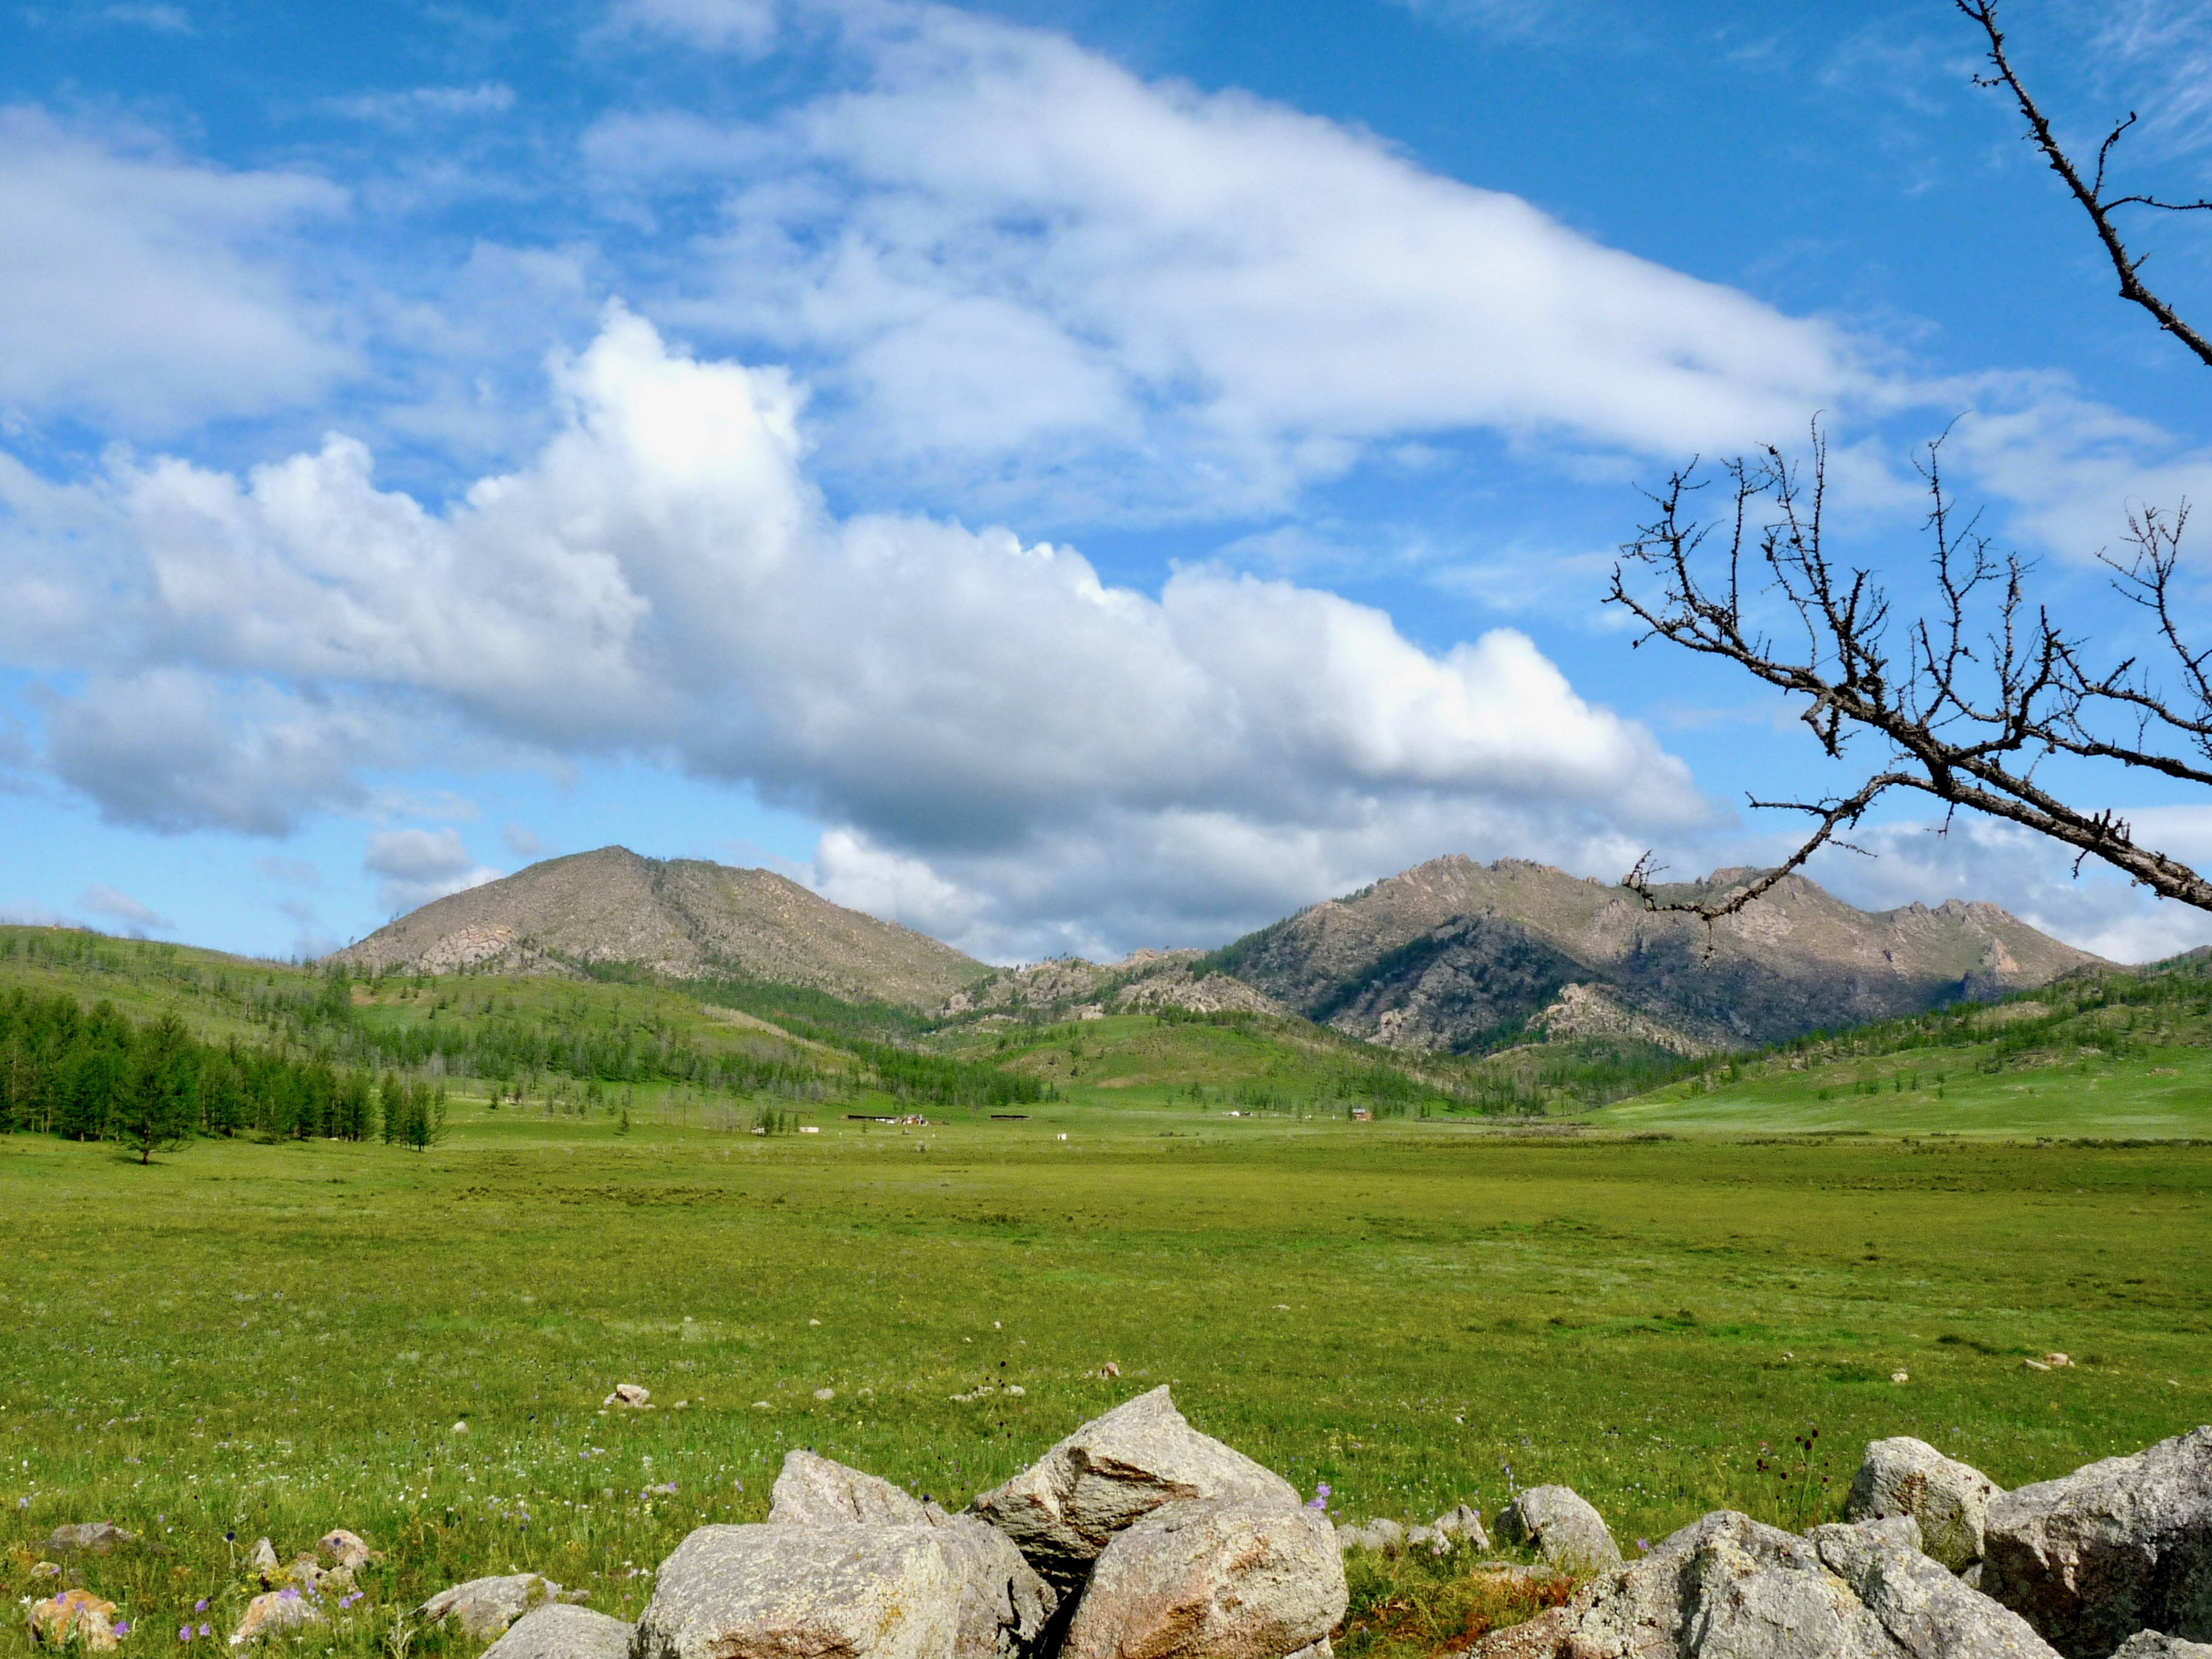
\includegraphics[height=303.00mm,width=431.22mm]{P1000675.jpeg}}
\rput[lb](0,0){\usebox\IBox}
% spine
%\psframe[fillstyle=solid,fillcolor=NavyBlue](213.00mm,0)(218.22mm,303.00mm)
% front

%\newsavebox\Titlebox
%\sbox\Titlebox{
%\fcolorbox{black}{white}{
%\begin{minipage}{110.00mm}
%\begin{center}
%\vspace{19.05mm}
%{\Huge \textbf{\emph{C++ Code Snippets}}}
%
%\vspace{12.7mm}
%{\LARGE Michele Iarossi}
%\vspace{19.05mm}
%\end{center}
%\end{minipage}}
%}

\newsavebox\Titlebox
\sbox\Titlebox{
\begin{tcolorbox}[colback=white,%white background
                  colframe=black,% black frame colour
                  width=12.2cm,% Use 11cm total width,
                  arc=3mm, auto outer arc,
                 ]
\begin{minipage}{110.00mm}
\begin{center}
\vspace{10.05mm}
{\Huge \textbf{\emph{C++ Code Snippets}}}

\vspace{12.7mm}
{\LARGE \emph{Michele Iarossi}}
\vspace{10.05mm}
\end{center}
\end{minipage}
\end{tcolorbox}
}
\rput[lb](266.22mm,190.5mm){\usebox\Titlebox}

% QR code
\newsavebox\QRbox
\sbox\QRbox{
\fcolorbox{black}{white}{
\begin{minipage}{38.1mm}
\begin{center}
\vspace{3.81mm}
\begin{pspicture}(25mm,25mm)
\psbarcode{http://www.mathsophy.com}{eclevel=H width=1.0 height=1.0}{qrcode}
\end{pspicture}
\texttt{{\small www.mathsophy.com}}
\end{center}
\end{minipage}}
}
\rput[lb](152.4mm,25.4mm){\usebox\QRbox}
\end{pspicture}
\end{document}
